\chapter{Hardware}
To carry out the commanded motion, the desired platform velocity vector is mapped into individual wheel angular velocities through an inverse Jacobian transformation:

\[
\dot{\mathbf{q}} = J^{-1} \cdot \dot{\mathbf{P}}
\]

In this expression, $\dot{q} \in R^4$ is the vector of angular velocities of the four drive wheels, while $\dot{P} \in R^3$ is the platform velocity vector consisting of the forward velocity $V_x$, lateral velocity $V_y$, and yaw rate $\dot{\theta}_z$. The inverse Jacobian matrix $J^{-1}$ relates the platform motion to the required wheel speeds, based on the robot's kinematic configuration.

For the X-drive configuration, the Jacobian takes the following matrix form:

\begin{figure}[H]
\[
\begin{bmatrix}
\dot{q}_1 \\
\dot{q}_2 \\
\dot{q}_3 \\
\dot{q}_4 \\
\end{bmatrix}
=
\frac{1}{r}
\begin{bmatrix}
-\sin(\theta + \frac{\pi}{4}) & \cos(\theta + \frac{\pi}{4}) & R \\
-\sin(\theta + \frac{3\pi}{4}) & \cos(\theta + \frac{3\pi}{4}) & R \\
-\sin(\theta + \frac{5\pi}{4}) & \cos(\theta + \frac{5\pi}{4}) & R \\
-\sin(\theta + \frac{7\pi}{4}) & \cos(\theta + \frac{7\pi}{4}) & R \\
\end{bmatrix}
\begin{bmatrix}
V_x \\
V_y \\
\dot{\theta}_z \\
\end{bmatrix}
\]
\caption{Wheel velocity calculation using the inverse Jacobian matrix. The vector on the left-hand side \( [\dot{q}_1, \dot{q}_2, \dot{q}_3, \dot{q}_4]^T \) represents the angular velocities of the four wheels. The Jacobian matrix reflects the X-drive wheel configuration. In this context, \( \theta \) is the robot's global orientation, \( R \) is the radial distance from the robot's centre to each wheel, and \( r \) is the wheel radius. The input vector on the right-hand side comprises \( V_x \) and \( V_y \), the body-frame linear velocities, and \( \dot{\theta}_z \), the angular velocity about the vertical axis.}
\label{fig:matrix-wheel}
\end{figure}

Each resulting wheel angular velocity \( \dot{q}_i \) is then used as a target input to a local PID controller, which ensures the wheel reaches and maintains this desired velocity. The control law is based on the difference between the target and measured angular velocities of the wheel:

\[
e_i(t) = \dot{q}_i^{\text{target}}(t) - \dot{q}_i^{\text{measured}}(t)
\]

The control input \( u_i(t) \), which is applied to the motor driver, is then computed using the standard PID formulation:

\[
u_i(t) = K_p e_i(t) + K_i \int_{0}^{t} e_i(\tau)\, d\tau + K_d \frac{d}{dt} e_i(t)
\]

Here, \( e_i(t) \) represents the instantaneous control error at time \( t \), \( K_p \) is the proportional gain that reacts to present error, \( K_i \) is the integral gain that accumulates past error to eliminate steady-state offset, and \( K_d \) is the derivative gain that anticipates future error trends. The PID controller thus dynamically adjusts the motor actuation to match the target wheel velocity, enabling precise and stable tracking of the robot's motion commands.

\section{Base Platform Modification and Microcontroller Integration}
The initial version of the robot was built using Dynamixel AX-12W motors. However, we encountered major issues in odometry due to the low quality and unreliability of the built-in encoders. These limitations hindered accurate velocity and position estimation.

To overcome these issues, we redesigned the robot base. The new design incorporates DC motors equipped with optical encoders mounted on the rear shaft. This design offers improved resolution and provides reliable velocity feedback, which is crucial for accurate closed-loop control.

Figure~\ref{fig:encoder-mounting} shows the configuration, where four DC motors operate in coordination. Each motor is driven by an L298N H-bridge motor driver. The control signals for each driver are generated by an ESP32 microcontroller.

\begin{figure}[H]
    \centering
    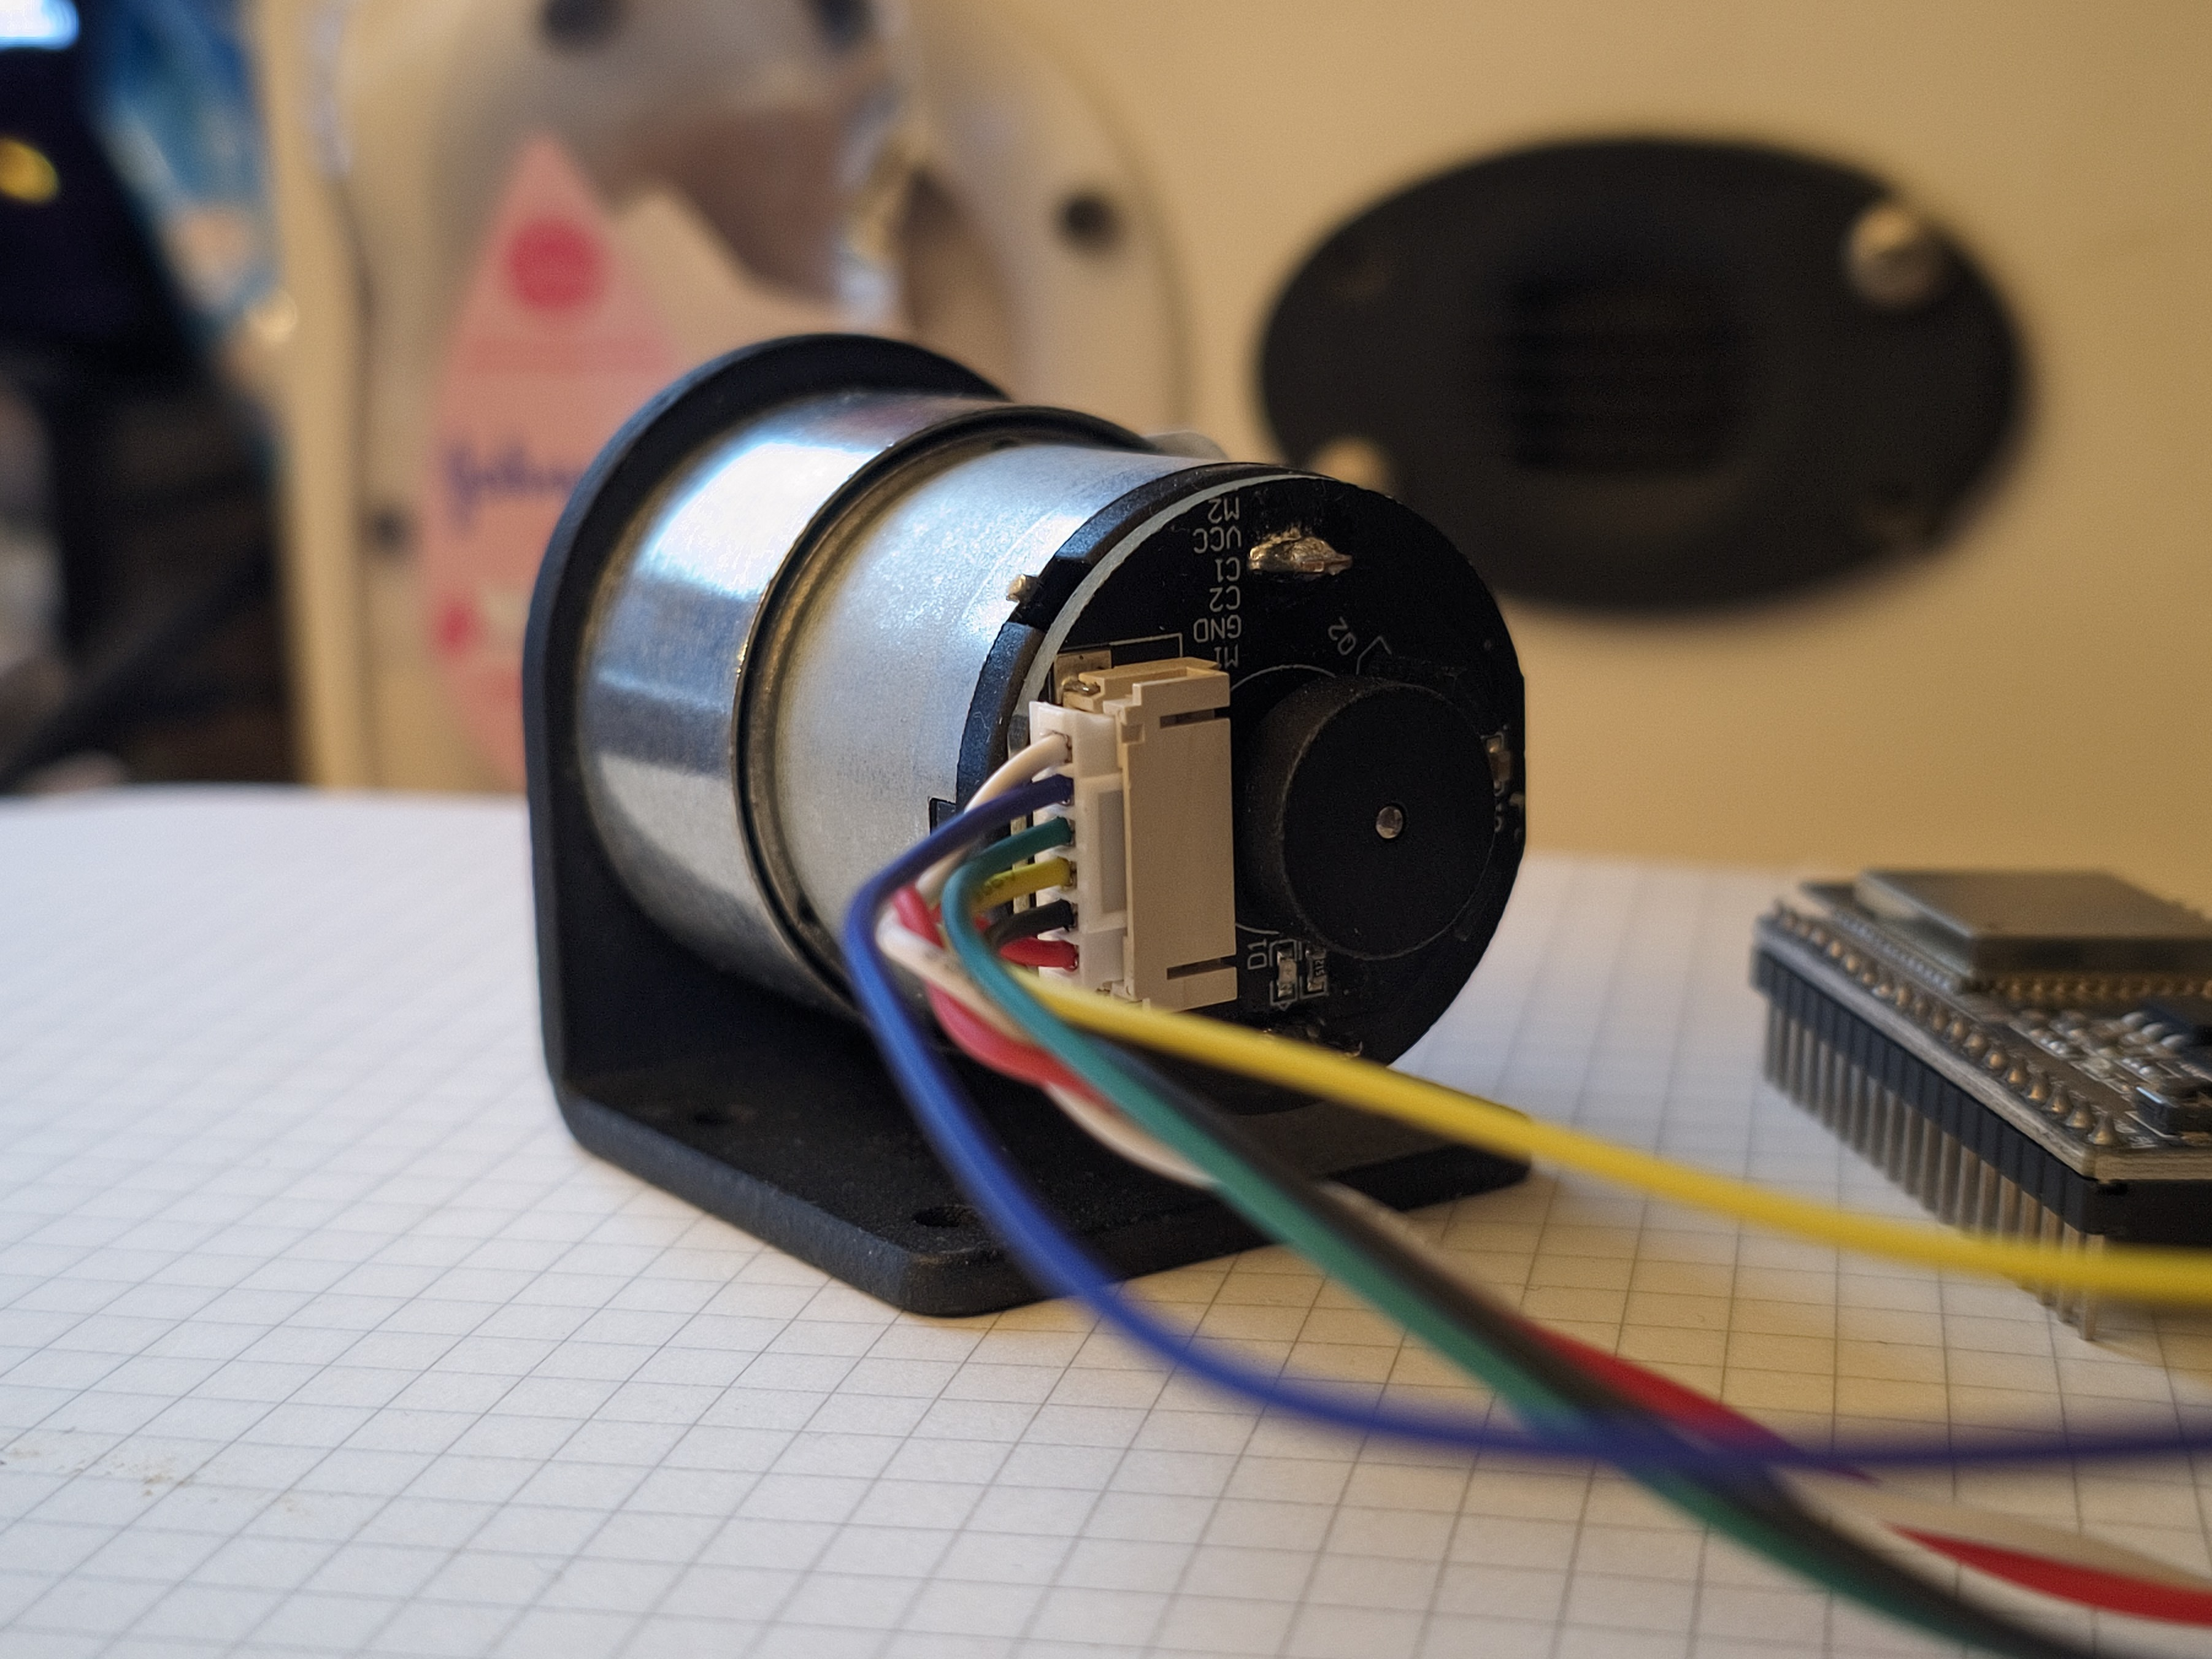
\includegraphics[width=0.6\textwidth]{assets/images/hardware/img2.jpeg}  % Replace with actual path
    \caption{DC motor with integrated encoder at the rear shaft, enabling closed-loop control.}
    \label{fig:encoder-mounting}
\end{figure}

The ESP32 is programmed using the ESP-IDF framework, which is based on FreeRTOS. Unlike the Arduino framework, ESP-IDF provides direct access to low-level resources and supports real-time scheduling. This choice removes the overhead introduced by Arduino’s abstraction layers and enables finer control over timing and concurrency. As a result, we achieve more accurate and responsive motor control.

The new platform design and software stack lay the foundation for the following section, which describes the detailed architecture of the motor control system.